
\documentclass[aps,twocolumn,secnumarabic,balancelastpage,amsmath,amssymb,nofootinbib, floatfix]{revtex4-2}

%%%%%%%%%%%%%%%%%%%%%%%%%%%%%%%%%%%%%%%%%%%%%%%%%%%%%%%%%%%%%%%%%%%

\usepackage{float}
\usepackage{graphicx}      % tools for importing graphics
%\usepackage{lgrind}        % convert program code listings to a form 
                            % includable in a LaTeX document
%\usepackage{xcolor}        % produces boxes or entire pages with 
                            % colored backgrounds
%\usepackage{longtable}     % helps with long table options
%\usepackage{epsf}          % old package handles encapsulated postscript issues
\usepackage{bm}            % special bold-math package. usge: \bm{mathsymbol}
%\usepackage{asymptote}     % For typesetting of mathematical illustrations
%\usepackage{thumbpdf}
\usepackage[colorlinks=true]{hyperref}  % this package should be added after 
                                        % all others.
                                        % usage: \url{http://web.mit.edu/8.13}


%%%%%%%%%%%%%%%%%%%%%%%%%%%%%%%%%%%%%%%%%%%%%%%%%%%%%%%%%%%%%%%%%%%
% And now, begin the document...
%%%%%%%%%%%%%%%%%%%%%%%%%%%%%%%%%%%%%%%%%%%%%%%%%%%%%%%%%%%%%%%%%%%

\begin{document}
\title{Measuring Planck's Constant in the Photoelectric Effect}
\author{Octavio Vega}
\email{ovega84@mit.edu}
%\homepage{http://web.mit.edu/8.13/} %If you don't have one, just comment out this line.
\date{\today}
\affiliation{MIT Department of Physics}

\begin{abstract}
In this experiment, we observe the photoelectric effect and measure Planck's constant. We seek to determine a relationship between the retarding voltage required to extinguish photocurrents and the frequency of the incident light on the metal surface from which electrons are ejected. We measure photocurrents produced in the presence of a retarding voltage which we vary incrementally for six different band-pass filters of unique central wavelengths. After finding the cutoff voltages which yield zero current, we consider a linear relationship between stopping voltages of photocurrents and frequency of incident light on a potassium surface. The slope of this line, determined via linear regression, leads us to the value of $h$. We calculate a value of $h=\left(5.0112\pm 1.5302\pm 0.1603\right) \cdot 10^{-34}$ joules-seconds for Planck's constant. 
\end{abstract}

\maketitle


%%%%%%%%%%%%%%%%%%%%%%%%%%%%%%%%%%%%%%%%%%%%%%%%%%%%%%%%%%%%%%%%%%%%%%%%
\section{Problem and Relevant Theory}

%\subsection{Expository Writing}
The photoelectric effect is the process by which electromagnetic radiation of sufficiently high energy excites the electrons in the atoms of a metallic surface such that they are ejected from the metal with some kinetic energy. 

Planck's constant is a physical constant of especially high significance; as per Max Planck, this is the constant of proportionality by which we may relate the frequency of electromagnetic radiation to its energy via the relation $E=h\nu$. This same relationship is crucial to understanding one of the earliest postulates of quantum mechanics, which is that radiation does not come in a continuous spectrum but rather in packets known as 'quanta' with energy specified by the above equation. 

By conservation of energy, we have the following relationship:
$$K = h\nu - \phi$$ where
\begin{itemize}
	\item K is the kinetic energy with which the electron leaves the metal's surface,
	\item $h$ is Planck's constant, $6.626\cdot 10^{-34}$ J$\cdot$s, 
	\item $\phi$ is the work function of the metal, which is material specific and represents the barrier energy which must be overcome in order for light to successfully remove electrons from the surface,
	\item $\nu$ is the frequency of the incident light, also given by the relation $c=\lambda\nu$, where $c$ is the constant speed of light and $\lambda$ is the wavelength of incident light.
\end{itemize}

We also note that electrons are charged particles, with charge given by $e=-1.602\cdot10^{-19}$ Coulombs, and therefore gain energy when accelerated across electric fields created by potential differences. In this experiment, we make use of retarding voltages to apply counteractive electric fields to hinder the electrons in their path. We can quantify the amount of energy an electrons gains (or loses) in an elecric field by $$K=e\int_{x_{i}}^{x_{f}}\vec{E}\cdot d\vec{x}=eV$$ where $V$ is the retarding voltage generating the electric field. Hence, substituting this into our conservation of energy relatioship and dividing through by the electron charge, we find
$$V=\frac{h}{e}\nu-\frac{\phi}{e}$$

\begin{figure}[H]
	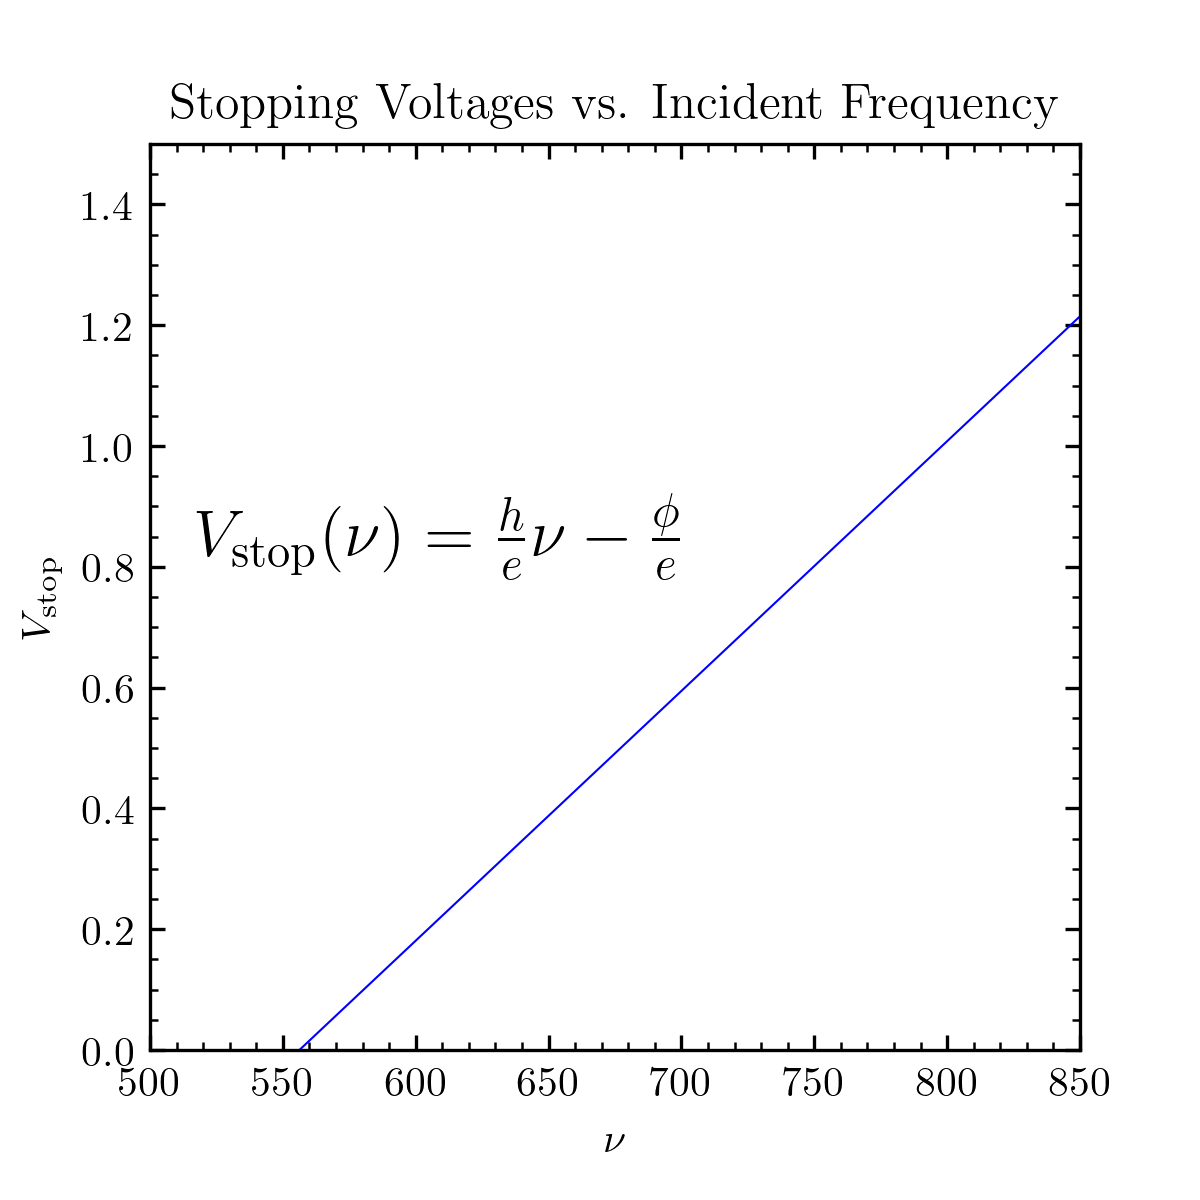
\includegraphics[width=9cm]{sample_stopping_volts.png}
	\caption{A sample plot of stopping voltage varying with frequency of incident light.}
	\label{fig:model}
\end{figure}

This linear relationship serves as our model in computing Planck's constant, which here is given by the slope of this linear relationship times the electron charge. In Figure~\ref{fig:model}, I provide an example of what this theoretical model of stopping voltage as a function of incident frequency will look like. 



%%%%%%%%%%%%%%%%%%%%%%%%%%%%%%%%%%%%%%%%%%%%%%%%%%%%%%%%%%%%%%%%%%%%%%%%
\section{Experimental Sketch and Salient Details}

\begin{figure}[H]
	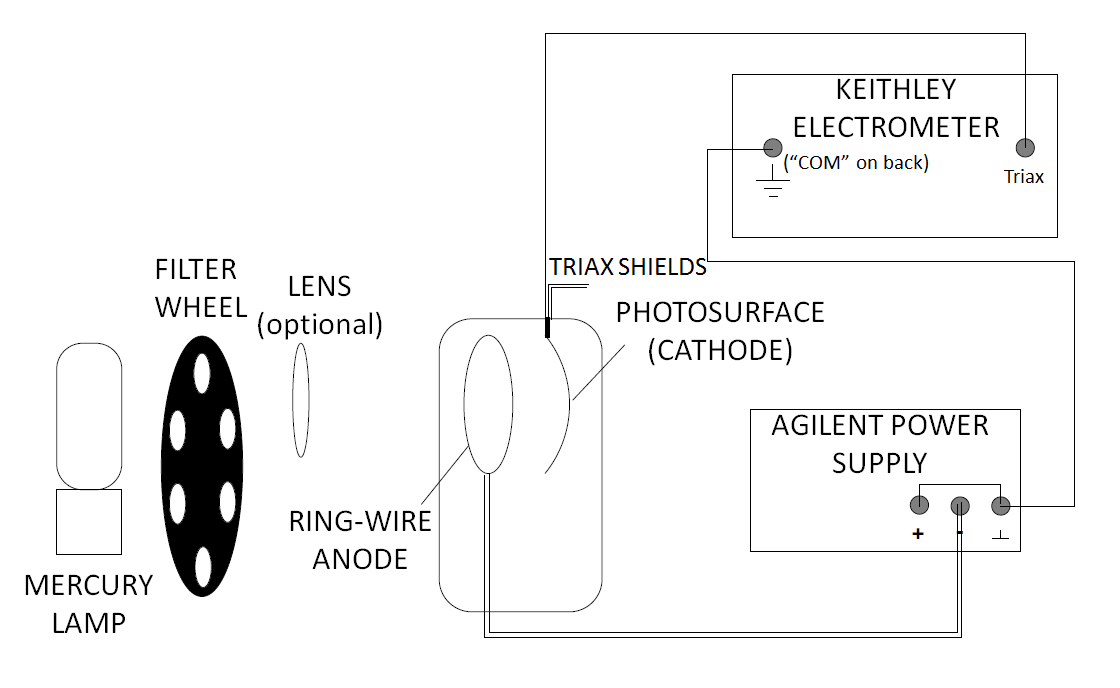
\includegraphics[width=9cm]{apparatus_setup.png}
	\caption{A schematic of the main apparatus. An issue is that the distance between the mercury lamp and the photosurface is not fixed; the latter rests on a rail which is adjustable, therefore providing more space for error. Taken from the Junior Lab photoelectric effect lab manual \cite{photoeffect}}.
	\label{fig:apparat}
\end{figure}

Our apparatus consisted of the following components:
\begin{itemize}
	\item Mercury lamp: We used a high power mercury discharge lamp as our source of radiation. This light served as the incident electromagnetic radiation on the metal surface. 
	\item Filter wheel: This wheel functioned as a selector for different frequencies. Each aperture on the wheel is a band-pass filter that allows a unique central wavelength, and thereby unique frequency, of light to pass through. This was how we varied the incident frequency. 
	\item Lens: The lens, which was an optional component, focused the incoming light to avoid striking the cathode ring and reaching the photosurface more precisely. 
	\item Ring wire anode: The anode was ring shaped to prevent the incident light from striking it, which would thereby detract from any detected photocurrent as it was held at negative potential relative to the cathode. The anode was made out of a platinum-rhodium alloy.
	\item Photosurface: The photosurface, also functioning as the cathode, was made from an oxidized silver coating onto which a thin layer of potassium was deposited, all connected to the brass cap on top of the photocell. This was the metal surface off of which photoelectrons are ejected.
	\item Power supply: We used an Agilent power supply to create a retarding voltage against the photocurrent, which we were able to vary directly.
	\item electrometer: We used a Keithley electrometer to observe measured photocurrents emanating from the photosurface in units of nanoamperes (nA). The electrometer required triaxial grounding in order to be double grounded.
\end{itemize}
A diagram of the apparatus with the above components labeled is provided in Figure~\ref{fig:apparat}. 

To determine stopping voltages, our procedure was as follows. We varied the input retarding voltage on the power supply incrementally up from 0 volts. After collecting numerous data points of retarding voltage versus photocurrent, we increased the retarding voltage until the resulting photocurrent was near zero nanoamps. At this point, we varied the retarding voltage around a small neighborhood of this point and determined the stopping voltage to within $\pm0.01$ volts.
%%%%%%%%%%%%%%%%%%%%%%%%%%%%%%%%%%%%%%%%%%%%%%%%%%%%%%%%%%%%%%%%%%%%%%%
\section{Data Presentation and Error Analysis}


In this section I present raw data collected, as well as our reduced data followed by a discussion on the relevant errors and their sources. 

\subsection{Variation of Photocurrent with Retarding Voltage}

\begin{figure}[H]
	\centering
	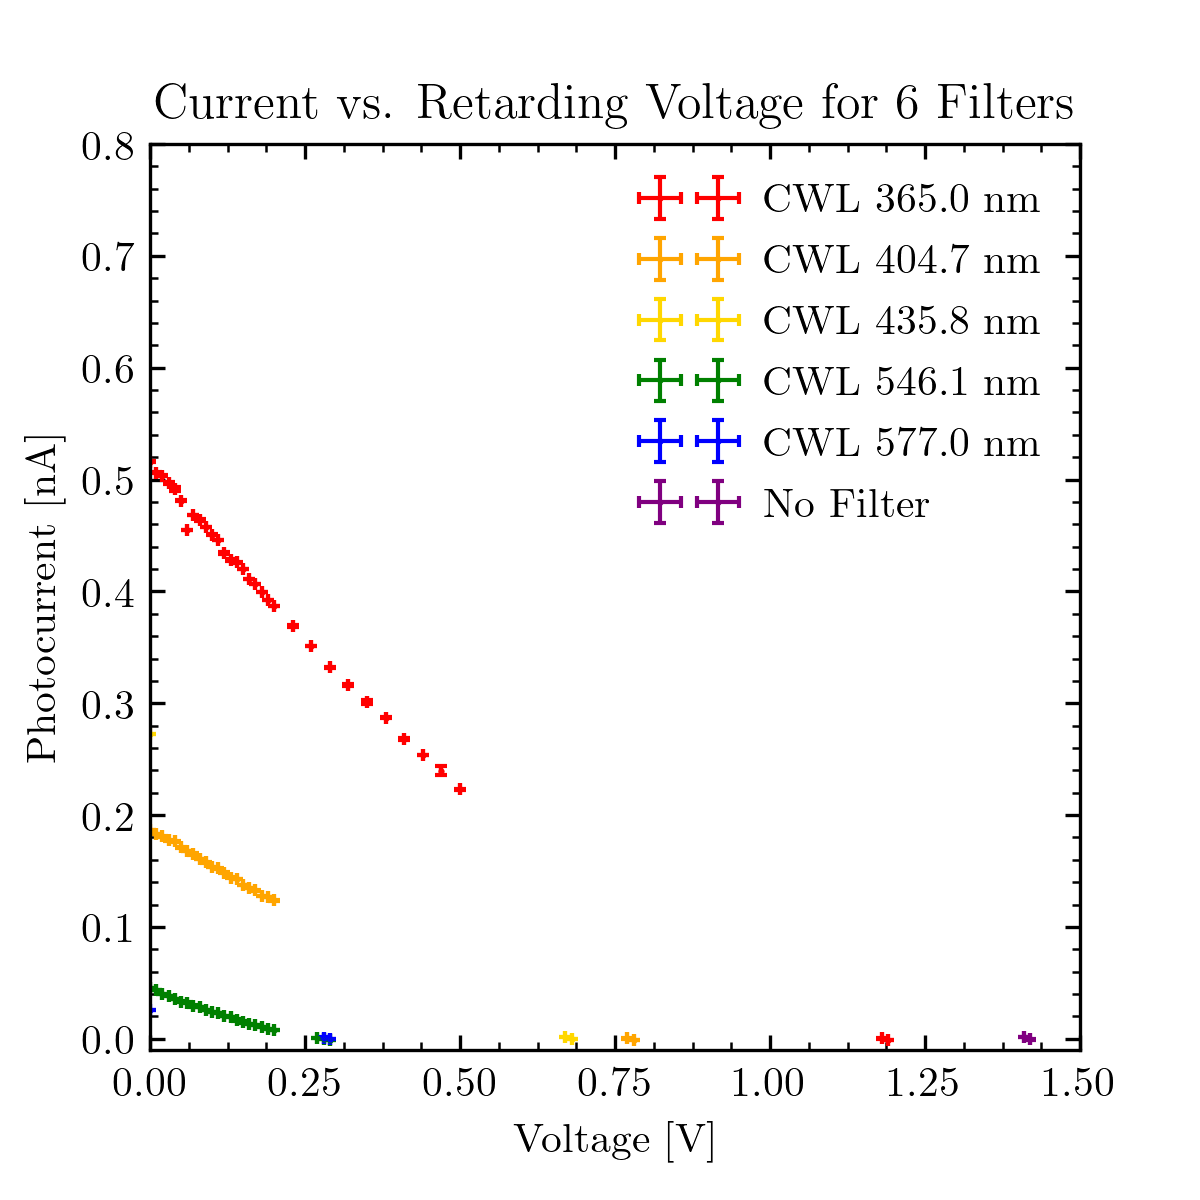
\includegraphics[width=9cm]{all_lenses_scatter.png}
	\caption{The variation of photocurrent with retarding voltage across six different filters.}
	\label{fig:allfilters}
\end{figure}

We used 6 filters in this experiment, 5 of which were separate filters with distinct central wavelengths (CWL) and the sixth of which was simply no filter, allowing incident light to travel through unhindered. In figure~\ref{fig:allfilters} I plot all of the data we gathered across each of the six filters for levels of photocurrent detected in nanoamperes as we varied the retarding voltage. 

As expected, the band-pass filters with the lowest central wavelength, and therefore the highest allowed frequency of incident light, corresponded to higher measured photocurrents at the same retarding voltage. This matched our intuition that greater frequency provides a higher intensity of light on the area of the metal surface, increasing the rate of electrons ejected. 

We also see features near the horizontal zero axis, which are disjoint from the points at the lower end of the retarding voltage spectrum. This is because we decided to stop taking data after varying the retarding voltage from zero up to a certain point, and simply skip to voltages that approximate the point at which detected photocurrent drops to zero so as to determine this stopping voltage more quickly. These small features near the bottom of the plot corresponded to our measurements of photocurrent near each filter's respective cutoff voltage. 


\begin{figure}[H]
	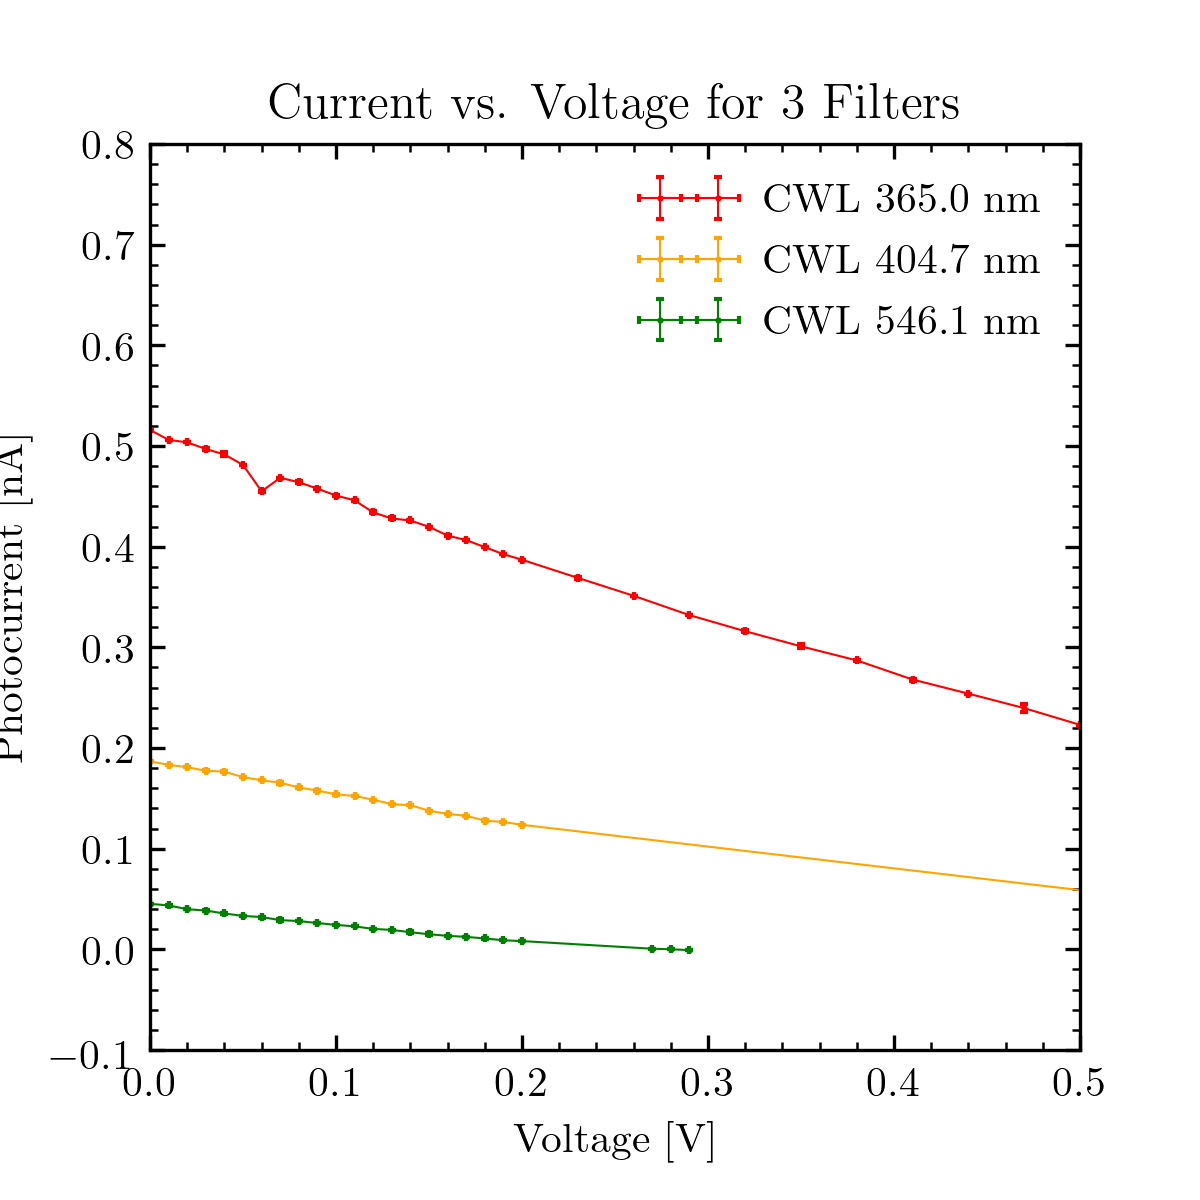
\includegraphics[width=9cm]{4_lenses_scatter.png}
	\caption{The variation of photocurrent with retarding voltage for  3 filters.}
	\label{fig:4filters}
\end{figure}
 

\begin{figure}[H]
	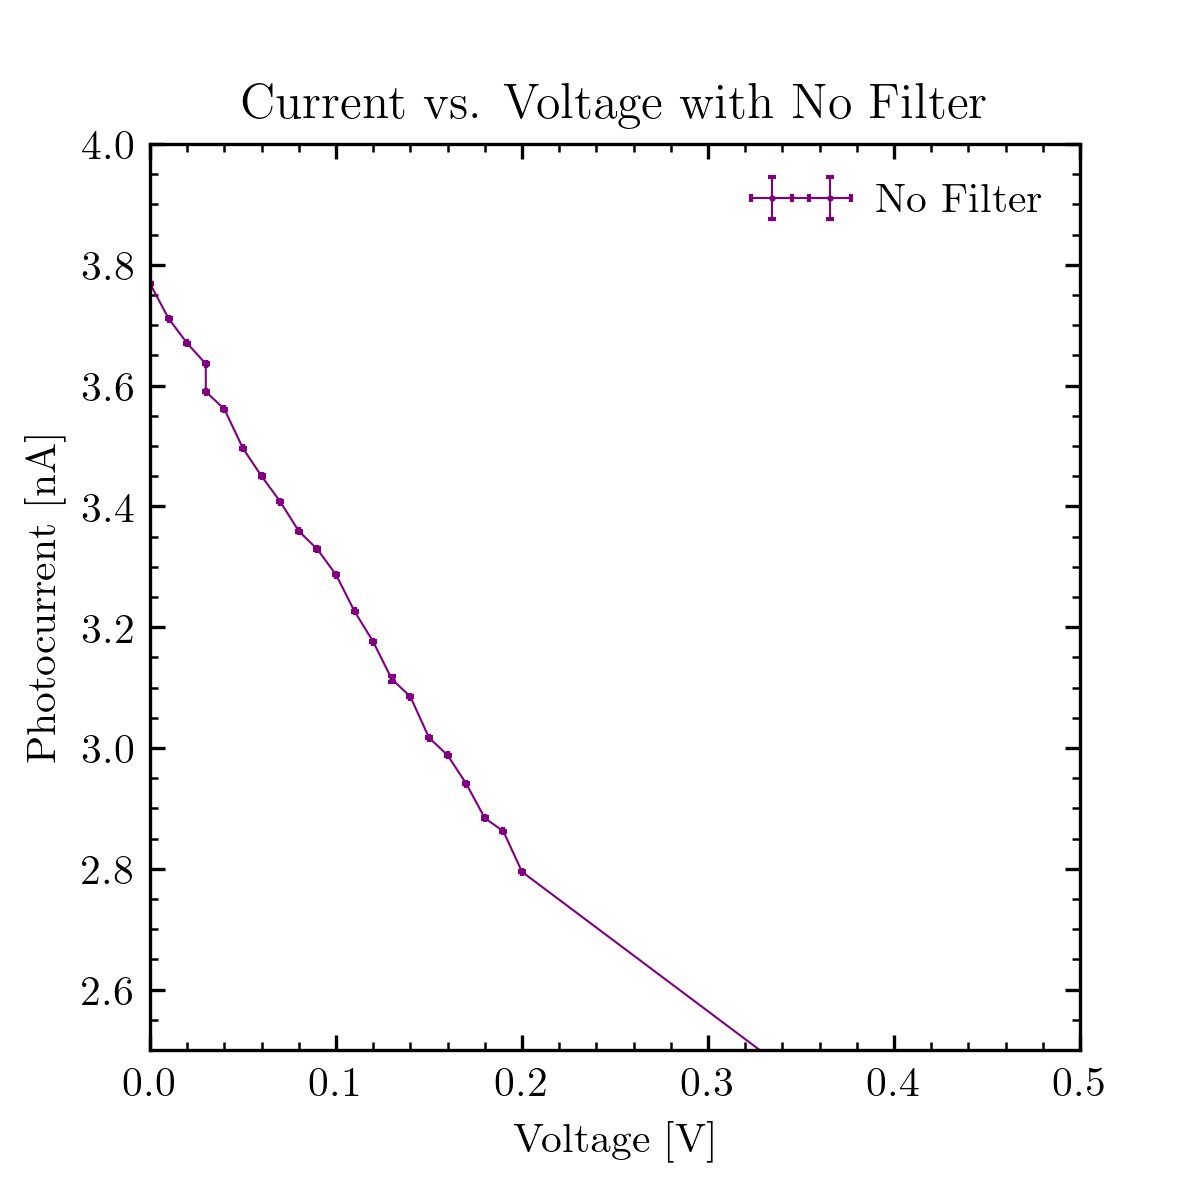
\includegraphics[width=9cm]{nolens_scatter.png}
	\caption{The variation of photocurrent with retarding voltage when no filter is present.}
	\label{fig:nofilter}
\end{figure}

I also compare the photocurrent vs. retarding voltage relationships across 3 of the filters with the data collected for the situation in which there is no filter, as seen in figure~\ref{fig:4filters} and in figure~\ref{fig:nofilter}.

\subsection{Comparing Stopping Voltages} 

\begin{figure}[H]
	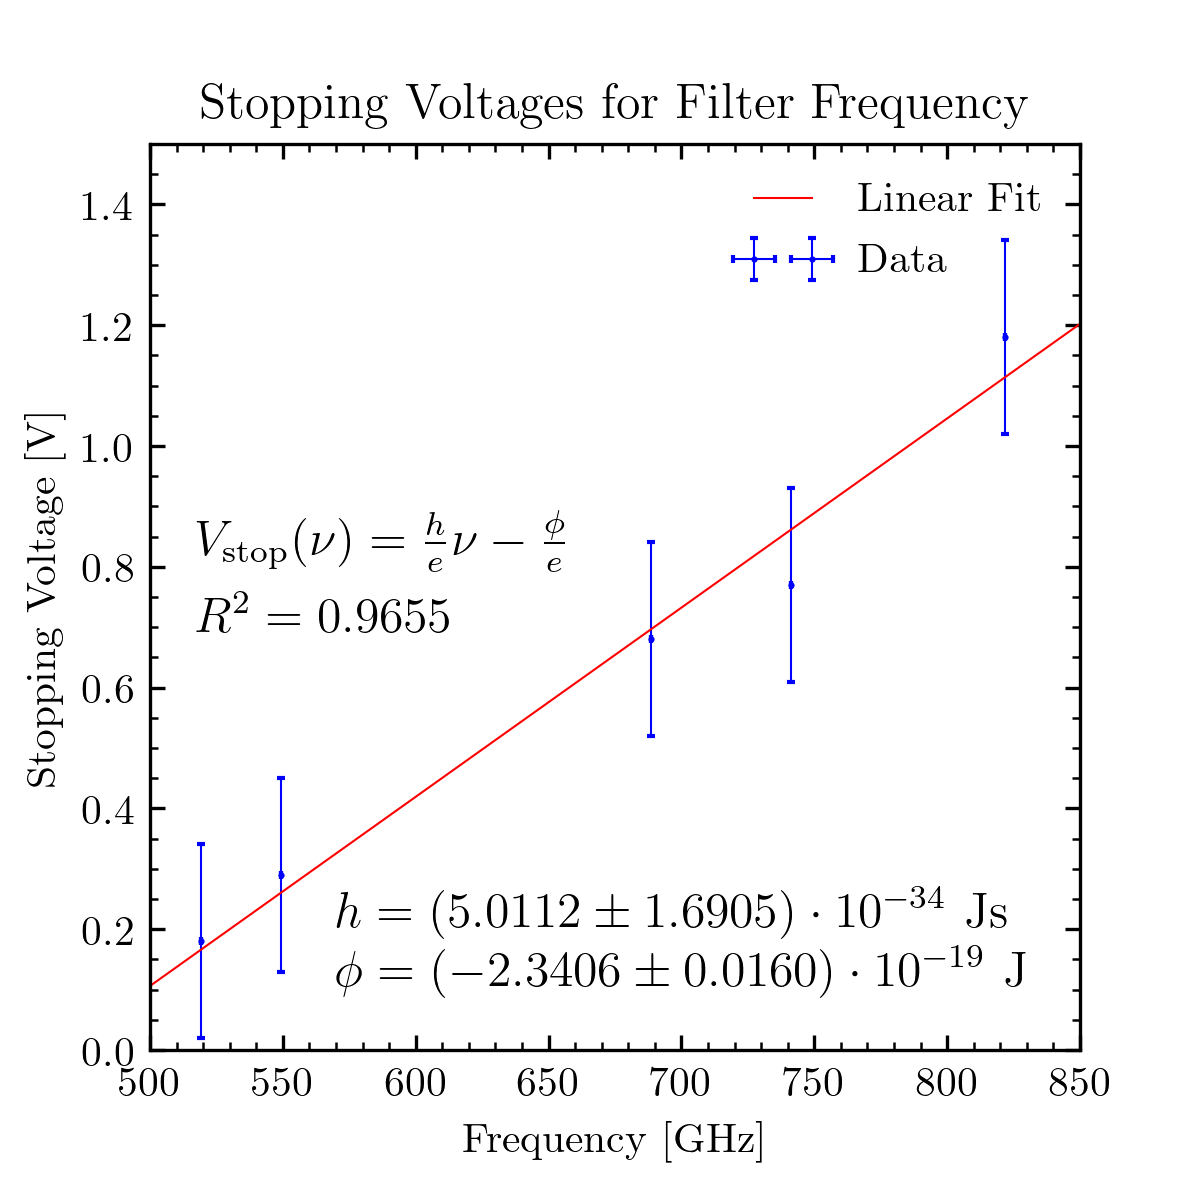
\includegraphics[width=9cm]{stopping_volts.png}
	\caption{A linear regression model fit to the stopping voltage vs. frequency data. The error bars represent the standard error of the data. The slope of the linear curve is equal to the ratio of Planck's constant to the electron charge, i.e. $\frac{h}{e}$.}
	\label{fig:stoppingvolts}
\end{figure}

After determining stopping voltages for each of the 5 distinct filters, I plot the stopping voltages against the filter frequencies in figure~\ref{fig:stoppingvolts}.

I fit a linear function to the data, whose slope is given by the ration $\frac{h}{e}$ and vertical intercept (not shown on the plot) is equal to $-\frac{\phi}{e}$. Multiplying the resulting slope from the fit by the charge $e$, I find a value for planck's constant of $h=(5.0112\pm 1.6905)\cdot 10^{-34}$ Js. Similarly, for the work function of the material, I find a value of $\phi=(2.3406\pm 0.0160)\cdot  10^{-19}$J.

\subsection{Error Estimation and Discussion}
I estimate the statistical uncertainties and systematic uncertainties in my measurement of $h$ to be $0.1603\cdot10^{-34}$ and $1.5302\cdot10^{-34}$ Js, respectively. 

Due to the precision of the equipment used in this experiment, the statistical uncertainty is relatively low. Contrarily, the systematic error dominates the uncertainty of this measurement which corresponds to the inaccuracy in my value of $h$. 

I attribute the sources of the systematic uncertainty to a number of factors:
\begin{itemize}
	\item Due to the inhomogenous metal surface, the work function is not uniform. Estimating it as such caused us to neglect the exact illumination of the metal surface area. The photodiode encasing may have shifted to an angle not directly in line with the incident radiation, for which we did not account. 
	\item The distance between the photodiode and the and the mercury radiation lamp was not held constant. Since data was acquired over two days in the laboratory, there is a high possibility that this value shifted between the two days, or even during data recording sessions. This uncertainty may have caused a different degree of illumination of the metal surface, or caused the incident radiation to strike the anode to a greater degree thereby offsetting the photocurrent. 
\end{itemize}  
Some additional sources of statistical errors include:
\begin{itemize}
	\item Lack of repeated trials: each of the six filters was used to collect data, but the stopping voltage was only determined once for each.
	\item Some minor fluctuations in the electrometer readings prevent an exact measurement of $V_{\mathrm{stop}}$. 
\end{itemize}
%%%%%%%%%%%%%%%%%%%%%%%%%%%%%%%%%%%%%%%%%%%%%%%%%%%%%%%%%%%%%%%%%%%%%%%
\section{Conclusions}
Ultimately, we find a value for $h$ within 24\% of the true value. The accuracy of our result might improve with more strict observation of sources of systematic uncertainty. Our data was taken under limited laboratory time, and thus could have been budgeted more effectively to allow for these adjustments. 

Broadly, we observe an increasing stopping voltage with increasing incident frequency as expected. Hence, we accurately observe the overall behavior of the photoelectric effect that matches our intutition. This relationship confirms the theory of the photoelectric effect and reinforces our understanding that waves do indeed behave as particles, in that in keeping with the physics of ellastic collisions, greater energy is required to eject electrons from a surface against stronger retarding voltages. 

%%%%%%%%%%%%%%%%%%%%%%%%%%%%%%%%%%%%%%%%%%%%%%%%%%%%%%%%%%%%%%%%%%%%%%%
\begin{acknowledgments} The author gratefully acknowledges Swapnil Garg for serving as his lab partner during this experiment. The author is also very thankful to Professor Fakhri and Hanzhen Lin for their helpful comments on his presentation. 
\end{acknowledgments}

%%%%%%%%%%%%%%%%%%%%%%%%%%%%%%%%%%%%%%%%%%%%%%%%%%%%%%%%%%%%%%%%%%%%%%%%% Place all of the references you used to write this paper in a file
% with the same name as following the \bibliography command
%%%%%%%%%%%%%%%%%%%%%%%%%%%%%%%%%%%%%%%%%%%%%%%%%%%%%%%%%%%%%%%%%%%%%%%

\bibliography{paper0}

\end{document}
